\documentclass[12pt, letterpaper, twoside]{article}
\usepackage[utf8]{inputenc}
\usepackage{titling}
\usepackage{amsmath}
\usepackage{mathtools}
\usepackage{cmsrb}
\usepackage[OT2,T1]{fontenc}
\usepackage[serbian]{babel}
\usepackage{amsmath}
\usepackage{tikz}
\usetikzlibrary{shapes,shadows,arrows}
\tikzstyle{line} = [draw, -stealth, thick]
\usepackage{graphicx}
\DeclareUnicodeCharacter{2212}{-}
\usepackage[export]{adjustbox}
\graphicspath{ {./images/} }
\makeatletter
\newcommand{\mathleft}{\@fleqntrue\@mathmargin0pt}
\newcommand{\mathcenter}{\@fleqnfalse}
\makeatother
\title{ % 
    Ensemble - Boosting Methods
    \\ }

\author{Emilija Mirković, Sanja Živanović}
\date{December 2022.}
\begin{document}
\maketitle
\begin{center}
\textbf{\large{ 1.1 Boosting Methods}} 

\end{center}
\hspace*{4ex} Ensemble methods are techniques that increase model precision (accuracy of results, predictions) by combining several different models in order to create one that is highly reliable.
There are several types of ensemble methods, and in this paper we will describe one of the most significant: \textbf{Boosting methods}.\\
\hspace*{4ex} Boosting belongs to the group of \textbf{Sequential Ensemble Techniques} that generate base learners in a sequence that promotes dependence between them. In this way, the performance of the model is further improved by increasing weights to learners that were previously misclassified. Boosting was originally designed to be used for classification problems, but it can also be used for regression problems.\\
\hspace*{4ex}Basically, model boosting is done by training the model by improving on the shortcomings of earlier versions of it. The idea behind the creation of this method was to create a procedure that would combine the results of multiple "weak" \space classifiers to create one powerful set of all that makes the least error of all (committee).
\begin{center}
\textbf{\large{1.1 \emph{AdaBoost}}} 
\end{center}
\hspace*{4ex}\emph{AdaBoost} (short for \emph{Adaptive Boosting}) is one of the most popular and widely used boosting algorithms.
The founders of this method, Yoav Freund and Robert Shapire (year 1995.) who originally named it \emph{"AdaBoost.M1."}, solved the difficulties of earlier boosting algorithms with this invention. 
\\\hspace*{4ex} Suppose we have a training set $\{x_i,y_i\}$ and each $x_i$ has a paired $y_i$ representing the output variable encoded with $y_i \in \{-1,1\}$. Also, a weak classifier $G(x)$ is given which makes a prediction and takes one of the values from the set $G(x_j)\in\{-1,1\}$ for each $x_j$. The idea is that for each round of training there is a new, improved classifier, so we will develop a set of weak classifiers over time $\{G_1,...G_T\}$.
\\\hspace*{4ex}Initially, all weights are set equally and in each round of training, the weights of the misclassified elements are increased, and more focus is invested in the more difficult (weighted) elements.
On the training set, the error is calculated as follows:\begin{equation}
\bar{err}=\frac{1}{N}\sum_{i=1}^{N}I(y_i\neq G(x_i))
\end{equation}
while the expected error rate on the following predictions is:\\
$E_{XY}I(Y\neq G(X))$.
\\
\\
\\\hspace*{4ex}In the scheme below we will describe the algorithm \emph{AdaBoost.M1}. In each round of training, weights are assigned to certain elements of the set, which is why we later call it a "weighted set".
Labels $G_1(x),...,G_M(x)$ denote classifiers for a certain training stage (each stage of training has its own improved classifier) trained on these sets.
\\
\\
\\
\begin{tikzpicture}[scale=2]
\tikzstyle{ann} = [draw=none,fill=none,right]
\matrix[nodes={draw, ultra thick, fill=blue!20},
        row sep=0.3cm,column sep=0.5cm] {
\node[draw,fill=red!30,ellipse,text width=2cm](1) 
  {training set $G_1(x)$}; &
\node[draw,fill=cyan!30,ellipse,text width=2cm](2)
  {weighted set $G_2(x)$}; &
\node[draw,fill=cyan!30,ellipse,text width=2cm](3)
  {weighted set $G_3(x)$}; &
\node[draw,fill=cyan!30,ellipse,text width=2cm](4)
  {weighted set $G_M(x)$};\\
};
\path [line] (1) -- (2);
\path [line] (2) -- (3);
\path [line] (3) -- (4);
\end{tikzpicture}
\\
\\
Here, we will introduce the coefficients $\alpha_i$ that indicate the contribution of the corresponding $G_i(x)$ in the sense that they give more influence to a more accurate classifier. Formula for the last (best) classifier obtained by the previously described procedure is:
\begin{equation*}
G(x)=sign [\sum_{m=1}^{M}\alpha_m G_m(x)]
\end{equation*}
\\
\textbf{The final prediction} is made by improving and combining the classifiers during this process. 
\\
At this point, we will introduce the term \textbf{weight}, mark them with $w_1, w_2,...,w_N$ and assume that they are initially set to: $w_i=1/N$. 
During this process, we apply them to each element of the training set $(x_i,y_i), i=1,2,...N$ and this is how the data is modified step by step.
\begin{center}
\large{\emph{1.1.1 Method}}
\end{center}
I) the classifier is trained on the data in the usual way\\
II) the classification algorithm is applied to weighted observations\\
III) previous applies to iterations $m=2,3,...M$\\
M) classifier performance $G_{m-1}(x)$: correctly classified observations have a reduced weight, while incorrectly classified ones have an increased weight 
\\ Observations that are difficult to classify correctly have a greater impact and as the procedure continues (the iterations alternate), the difference between them becomes more and more obvious. Therefore, new, time-improved classifiers will focus more on elements of the training set that were misclassified by their predecessors.
\begin{center}
\large{\emph{1.1.2 AdaBoost.M1.} algorithm}\\
\end{center}
Now we will describe the mathematical part of the functioning of the AdaBoost algorithm.\\\\
1. set initial weights $w_i=\frac{1}{N},i=1,...N$.\\\\
2. for values m=1,...,M:\\
\hspace*{4ex}(a)\space using the current weight $w_i$ adjust the classifier $G_m(x)$ on the training set; that current classifier is induced on difficult observations\\\\
\hspace*{4ex}(b)\space calculate the resulting weighted error rate:
\begin{equation*}
err_m=\frac{\sum_{i=1}^N w_i I(y_i\neq G_m(x_i))}{\sum_{i=1}^N w_i}
\end{equation*}\\
\hspace*{4ex}(c)\space determine the coefficients: $\alpha_m=\log(\frac{1-err_m}{err_m})$\\\\
\hspace*{4ex}(d)\space set: $w_i=w_i*\exp [\alpha_m I(y_i\neq G_m(x_i))], i=1,2,...N.$. Here, the individual weights of each observation are updated for the next iteration\\\\
3. calculating the final prediction: $G(x)=sign[\sum_{m=1}^M\alpha_m G_m(x)]$\\\\\\
The factor $\exp(\alpha_m)$ scales the weights of observations misclassified by $G_m(x)$.
In this way, such observations increase the influence for inducing the next classifier $G_{m+1}(x)$. \\
A weak classifier is one whose predictive power is little better than random guessing. The quality of this algorithm is that it greatly improves the weak classifier, i.e. reduces its error.
The figure below illustrates how the classifier's error rate decreases as the boosting iterations unfold.\\\\
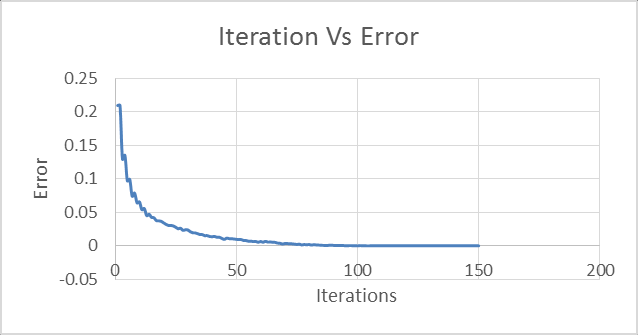
\includegraphics[width=13cm, height=7cm]{2}\\
\begin{center}
\textbf{\large{\\1.2 Boosting fits an Additive Model}\\}
\end{center}
Various classification and regression models can be represented as a linear combination of some simpler models. The formula for the generalized additive model is:
\begin{equation*}
f(x)=\sum_{m=1}^M \beta_m b_m(x;\gamma_m),
\end{equation*}
the variables in the previous model are:\\
- $x$ input data,\\
- $\{\beta_m,\gamma_m\}$ model parameters,\\
- $b_m(x;\gamma_m)$ are some arbitrary, simple functions with variable x\\\\
Amplification can be connected to additive models in that it represents a way of fitting additive expansion into a set of elementary functions (which in our case are the classifiers $G_m(x)\in\{-1,1\}$). In that case, the expansions of the elementary functions take the form of a generalized additive model.\\\\
How is the fitting of these models done?\\
-The model parameters $\{\beta_m,\gamma_m\}$ are estimated by minimizing a loss function (L, either quadratic or likelihood-based) that measures the prediction errors over the entire training set $\{x_n,y_n\}$:
\begin{equation*}
min_{\{\beta_m,\gamma_m\}_1^M} \sum_{i=1}^N L(y_i, \sum_{m=1}^M \beta_m b_m(x_i;\gamma_m)).
\end{equation*}
that is,
\begin{equation*}
\{\beta_m^*,\gamma_m^*\}_1^M=argmin_{\{\beta_m,\gamma_m\}_1^M}\sum_{i=1}^N L(y_i, \sum_{m=1}^M \beta_m b_m(x_i;\gamma_m)).
\end{equation*}
This calculation can be demanding, depending on the shape of the loss function and the basis functions $b_m(x;y)$.
\begin{center}
\textbf{\large{\\1.3 Forward Stagewise Additive Modeling}\\}
\end{center}
As already discussed, direct optimization of the loss function can be computationally challenging. However, if it is an alternative case where there is only one basic function, it can make our job a lot easier:
\begin{equation*}
min_{\beta,\gamma}\sum_{i=1}^N L(y_i,\beta b_m(x_i;\gamma)).
\end{equation*}
The idea behind forward stepwise modeling is to successively add new basis functions to approximate the solution of the original minimization problem:
\begin{equation*}
min_{\{\beta_m,\gamma_m\}_1^M} \sum_{i=1}^N L(y_i, \sum_{m=1}^M \beta_m b(x_i;\gamma_m)).
\end{equation*}
without changing the parameters that have been added.\\
The following algorithm will demonstrate the operation of forward stepwise modeling. It will be necessary to obtain a solution for the basis function $b(x;\gamma_m)$ and for the corresponding coefficient $\beta_m$ (in each iteration) which is then added to $f_{m-1}(x)$. In this way $f_m(x)$ is obtained and the process is repeated for the next iteration.\\
\begin{center}
\large{1.3.1 Forward Stagewise Modeling algorithm}\\
\end{center}
1. set $f_0(x)=0$.\\
2. for values of m from 1 to M:\\
\hspace*{6ex}(a)\space calculate:
\begin{equation*}
(\beta_m,\gamma_m)=argmin_{\beta,\gamma}\sum_{i=1}^N L(y_i,f_{m-1}(x_i)+\beta b(x_i;\gamma)).
\end{equation*}
\hspace*{6ex}(b)\space set $f_m(x)=f_{m-1}(x)+\beta_m b(x;\gamma_m)$\\\\
We will extract arguments of the loss function that we mentioned above $L(y_i,f_{m-1}(x_i)+\beta b(x_i;\gamma))$.\\
We distinguish between probability-based and squared-error loss functions. In the case of squared-error loss function, we set the well-known formula:
\begin{equation*}
L(y,f(x))=(y-f(x))^2,
\end{equation*}
and when the extracted arguments are inserted into this function we get:
\begin{equation*}
L(y_i,f_{m-1}(x_i)+\beta b(x_i;\gamma)) = (y_i-f_{m-1}(x_i)-\beta b(x_i;\gamma))^2,
\end{equation*}
Here, the most valuable addend is $\beta_mb(x;\gamma_m)$ which represents the residuals of this models residuals (or something close to residuals) and a
Ovde je najznačajniji sabirak $\beta_mb(x;\gamma_m)$ koji predstavlja reziduale ovog modela (ili nešto najbliže rezidualima) i dodaje se ekspanziji u svakoj iteraciji. Sa druge strane, prvi sabirak možemo obeležiti sa  $r_{im}=y_i-f_{m-1}(x_i)$ i on nam označava ostatak modela i-te observacije.\\\\
\begin{center}
\textbf{\large{\\1.4 Eksponential loss and boosting method \emph{AdaBoost} }\\}
\end{center}
How does the AdaBoost model fit into the whole story of the additive model and forward stagewise modeling?\\
-AdaBoost fits the additive model using stepwise modeling by:
\begin{itemize}
\item taking the binary classifier $G_m(x):R->\{-1,1\}$ for the elementary functions $b_m$
\item taking an exponential loss as the loss function
\end{itemize}
\begin{equation*}
L(y,f(x))=\exp(-y f(x))
\end{equation*}
Now that we know what the loss function looks like and what elementary functions are, we can solve the previously mentioned problems.
\begin{itemize}
\item We will start from a familiar expression
\begin{equation*}
(\beta_m,\gamma_m)=argmin_{\beta,\gamma}\sum_{i=1}^N L(y_i,f_{m-1}(x_i)+\beta b(x_i;\gamma)).
\end{equation*}
\item then insert known parameters
\begin{equation*}
(\beta_m,G_m)=argmin_{\beta,G}\sum_{i=1}^N \exp[-y_i(f_{m-1}(x_i)+\beta G(x_i))]
\end{equation*}
\item for the required weights configured in the expressions for the AdaBoost model (and applied to each observation), we will take $w_i=\exp(-y_i f_{m-1}(x_i))$
\item this is the correct form for the weight because it depends neither on the coefficient $\beta$ nor on the classifier $G(x)$
\begin{equation*}
(\beta_m,G_m)=argmin_{\beta,G}\sum_{i=1}^N w_i^{(m)} \exp(-\beta  y_i G(x_i)) (1.1)
\end{equation*}
\item the previous expression was derived in order to be able to add in each iteration the coefficient $\beta_m$ and the classifier $G_m$
\item In general, the weights in the AdaBoost model are different for each subsequent iteration. Considering that our chosen weights depend on the function $f_{m-1}(x_i)$, it can be concluded that the values of the weights themselves change as we go through the iterations (which was the initial idea)
\item now we need to split the data into two sets to decompose the sum above:
\item sada je potrebno da podelimo podatke u dva skupa da bismo razložili gornju sumu:
\begin{enumerate}
\item $I_1=\{y_i=G(x_i)\}$ 
\item $I_2=\{y_i\not=G(x_i)\}$
\end{enumerate}
\item dividing the sum into two
\begin{equation*}
(\beta_m,G_m)=argmin_{\beta,G}(e^{-\beta}\sum_{y_i=G(x_i)} w_i^{(m)} +e^{\beta}\sum_{y_i\not=G(x_i)}w_i^{(m)})
\end{equation*}
\begin{equation*}
(\beta_m,G_m)=argmin_{\beta,G}(e^{-\beta}\sum_{i=1}^N w_i^{(m)} +(e^{\beta}-e^{-\beta})\sum_{i=1}^N w_i^{(m)}I(y_i\not=G(x_i)))
\end{equation*}
\item in the previous equation, when we fix a value greater than zero of the coefficient $\beta_m$, we can obtain its solution and thus the expression of the optimal value for $G_m$
\end{itemize}
 \begin{equation*}
G_m=argmin_G\sum_{i=1}^N w_i^{(m)}I(y_i\neq G(x_i)) (1.2.)
\end{equation*}
This tells us that $G_m$ is actually a classifier that minimizes the weighted prediction error rate, given that the $w_i^{(m)}$ are weights assigned to the i-th element of the training set.\\
Now, naturally, we can also obtain the solution of equation 1.1 for the coefficient $\beta$.
\begin{itemize}
\item Let's go back to the expression
\begin{equation*}
(\beta_m,G_m)=argmin_{\beta,G}(e^{-\beta}\sum_{y_i=G(x_i)} w_i^{(m)} +e^{\beta}\sum_{y_i\not=G(x_i)}w_i^{(m)})
\end{equation*}
\item now we need to take the derivative with respect to the parameter $\beta$ and set it to zero in order to determine its minimum
\begin{equation*}
\frac{d(e^{-\beta}\sum_{y_i=G(x_i)} w_i^{(m)} +e^{\beta}\sum_{y_i\not=G(x_i)}w_i^{(m)})}{d\beta_m} = 0
\end{equation*}
\item the solution for $\beta$ is:
\end{itemize}
\begin{equation*}
\beta_m=\frac{1}{2}\log \frac{1-err_m}{err_m} (1.3)
\end{equation*}
where $err_m$ is the minimized weighted error rate
\begin{equation*}
err_m=\frac{\sum_{i=1}^N w_i^{(m)}I(y_i\neq G_m(x_i))}{\sum_{i=1}^N w_i^{(m)}}. (1.4)
\end{equation*}
Now it is necessary to examine the rule for updating weights, that is, how they change through iterations
\begin{equation*}
 \begin{aligned}
w_i^{(m+1)} &=exp(-y_if_m(x_i))\\
& =exp(-y_i(f_{m-1}(x_i)+\beta_mG_m(x_i)))\\
& =w_i^{(m)}exp(-\beta_m y_i G_m(x_i))\\
& =w_i^{(m)}exp(2\beta_mI(y_i\not=G_m(x_i)))exp(-\beta_m)
\end{aligned}
\end{equation*}
Now we go back to the \emph{AdaBoost} algorithm once we have gone through all its elements (we know where they come from):
\begin{enumerate}
\item we set the value for the weights $w_i=\frac{1}{N},i=1,...,N$
\item for m values from 1 to M:\\
\hspace*{4ex}(a) using the current weight $w_i$, adapt the classifier $G_m(x)$ on the training set\\
\hspace*{4ex}(b)\space determine the resulting weighted error rate:
\begin{equation*}
err_m=\frac{\sum_{i=1}^N w_i I(y_i\neq G_m(x_i))}{\sum_{i=1}^N w_i}
\end{equation*}\\
\hspace*{4ex}(c)\space determine the coefficients: $\alpha_m=\log(\frac{1-err_m}{err_m})$\\\\
\hspace*{4ex}(d)\space update the weights so that the following expression holds:\\ \hspace*{6ex}$w_i=w_i*\exp [\alpha_m I(y_i\neq G_m(x_i))], i=1,2,...N.$.
\item calculating the final prediction (algorithm output): $G(x)=sign[\sum_{m=1}^M\alpha_m G_m(x)]$
\end{enumerate}
It can be noted that we have taken $\alpha_m=2\beta_m$ for ease of notation.\\ 
From all of the above, we conclude that \emph{AdaBoost.M1} minimizes the exponential loss criterion $L(y,f(x))=\exp(-yf(x))$ using additive forward modeling.\\
\begin{center}
\textbf{\large{1.5 Other loss functions and Motivation for choosing Exponential Loss }\\}
\end{center}
By using exponential loss we can almost always get a simple AdaBoost algorithm and that is the main reason we choose it.\\
We will now examine what exactly it is assessing.
[Fridman paper, year 2000.] It can be shown that:
\begin{equation*}
f^*(x)=argmin_{f(x)}E_{Y|x}(e^{-Yf(x)})=\frac{1}{2}\log\frac{P(Y=1|x)}{P(Y=-1|x)},
\end{equation*}
from here we can get the probability that Y is correctly classified, i.e. that it is valid:
\begin{equation*}
P(Y=1|x)=\frac{1}{1+e^{-2f^*(x)}}.
\end{equation*}
The AdaBoost algorithm gives us half the logarithmic chance that Y will take the value 1. Furthermore, this justifies the use of its sign for the final classifier
\begin{equation*}
G_M(x) -> G(x)=sign [\sum_{m=1}^{M}\alpha_m G_m(x)].
\end{equation*}
The choice of the loss function is closely related to the complexity of the calculation and the robustness of the algorithm itself.The following loss functions can be used for classification:
\begin{itemize}
\item \textbf{0/1 loss}: $I\{sign(f(x))\not=y\}$
\item \textbf{binomial deviation}: $log(1+exp(-2yf))$
\item \textbf{loss of soft margin}: $(1-yf)I\{yf>1\}$ (SVM algoritham is used for this case)
\item \textbf{exponential loss} $exp(-yf(x))$ (AdaBoost algorithm is used in this case)
\end{itemize}
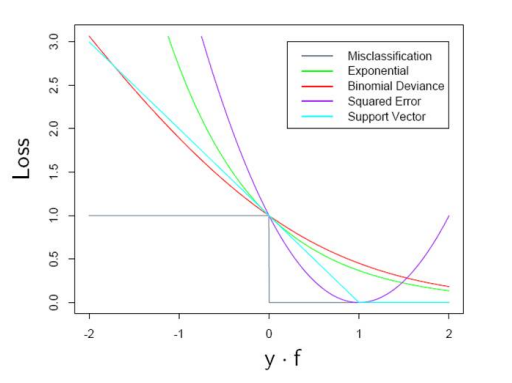
\includegraphics[width=11cm, height=7cm]{3}
\\\\"Loss" present a misclassification.\\
The following loss functions can be used for regression:\begin{itemize}
\item \textbf{squared error loss}: $(y-f(x))^2$
\item \textbf{an absolute loss}: $|y-f(x)|$
\item \textbf{Huber's loss}: $L(y,f)=$
\begin{enumerate}
\item \hspace*{10ex} $(y-f(x))^2$, ako je $|y-f(x)|<\delta$
\item \hspace*{10ex}$\delta(|y-f(x)|-\frac{\delta}{2})$, otherwise
\end{enumerate}
\end{itemize}  
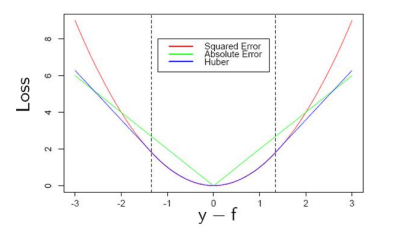
\includegraphics[width=11cm, height=7cm]{4}




\begin{center}
\textbf{\large{2 Loss Functions}} 

\end{center}
We will now examine the loss functions from the previous chapter in more detail.\\
Let $X \in R^{p}$ be the input data vector and $Y \in R$ the output variable, with joint distribution $F(X,Y)$. In decision theory, the main motivation is to find the function $f(X)$ to predict the variable $Y$. Since there is an error in every prediction, a loss function,
\begin{center}
 $L(Y,f(X)$
\end{center} is introduced which tells us how much the actual data differs from the data obtained by the prediction. Basically, the loss function measures how good the prediction model is in terms of being able to predict the expected outcome. Consequently, it is always good when the loss function is as small as possible.\\
\hspace*{4ex}The best known and most used is the quadratic loss function, 
\begin{center}
$L(Y,f(X)) = (Y - f(X))^2$. 
\end{center}
For the quadratic loss function, the function $f(X)$ is found as follows:\[EPE(f) = E(Y-f(X))^2 = \int [y-f(X)^2] \,F(dx,dy),\]
where EPE is the root mean square error of prediction.
By switching to the conditional expectation, we get \[EPE(f) = E_XE_{Y|X}([Y-f(X)]^2|X)\]
As we want the minimum error, we need the minimum of this function, i.e. \[f(X)=argmin_cE_{Y|X}([Y-c]^2|X=x).\]
The minimum is reached for \[f(x)= E(Y|X=x).\]
For the absolute error, \(L(Y,f(X)) = |Y-f(X)|\), the minimum is not reached for the conditional expectation, but for the conditional median: \(m(Y|X)\).\\
\hspace*{4ex} Loss functions for classification represent the price paid for the inaccuracy of classification predictions (identifying which category a particular observation belongs to). Given $X \in R^d$ is the space of all possible input data, and $Y = \{−1, 1\}$ is the set of all outputs, i.e. predicted data. The goal of classification is to find the function $f(x) : X -> R$ that best predicts y for a given input. However, due to incomplete data or other factors, it is possible for the same input data to generate different output data, resulting in erroneous and inaccurate predictions. Therefore, a loss function is introduced that needs to be minimized.\\
\hspace*{4ex} Let $F$ be a statement. Then we define the indicator function: \[
    I(F)=
\begin{cases}
    1,& \text{if } F\\
    0,& \text{if }   \neg F
\end{cases}
\]
That is, the error function here is of the form \(L(Y,f(X)) = I(Y \neq f(X)) \). Both exponential $exp(-yf(x))$ and binomial $log(1+e^{-2Yf(x)})$ loss functions are often used.\\
\hspace*{4ex} It is possible, and often desirable, to choose different loss functions for different problems and data types. In practice, it happens that not all mistakes are equally important. For example, some classes may be considered more closely related than others, so misclassification between them is tolerable, while misclassification of unrelated classes is a problem. This is an example of a \textbf{\textit{cost sensitive classification}}.
\pagebreak

\begin{center}
\textbf{\large{3 Robustness}} 
\end{center}
\hspace*{4ex} A statistical method is robust if it is resistant to errors in the results that occurred in the process of inference and prediction. Different loss functions behave differently in the case of extreme data, i.e. data that are at the limits of acceptability.\\
\begin{center}
\textbf{\large{3.1 Robust Loss Functions for Regression}}
\end{center}

\hspace*{4ex} For regression problems, we have seen that squared and absolute error are most often used. The question arises as to which of these two to use for better performance. Since the solutions $E(Y|X = x)$ for the quadratic function and $m(Y|X)$ for the absolute function are the same for symmetric distributions, with such data it does not matter which error function we use. However, the quadratic function places greater emphasis on observations with large absolute residuals $|y_i − f(x_i)|$, thus it is less robust and its performance is significantly reduced compared to the absolute error function, in the case of distributions with a long tail. Also, they perform worse when there are a lot of outliers.\\
\begin{center}
\textbf{\large{3.2 Robust Loss Functions for Classification}}
\end{center}

\hspace*{4ex} We have already stated that exponential and binomial loss functions are used in the classification. For the joint population distribution these two loss functions have the same solution, however, this is not the case for final data sets. Both functions are monotonically decreasing in $yf(x)$. In a classification whose output is -1 or 1, $yf(x)$ has a similar role to residuals in regression. The classification rule $G(x) = sign[f(x)]$ implies that observations with positive $y_if(x_i) > 0$ are correctly classified, while observations with negative $y_if(x_i) < 0$ are incorrectly classified. The decision boundary is $f(x) = 0$. The goal of classification is to have more positive observations. Any loss function should "punish" \space negative observations more than "reward"\space positive ones, given that positive ones are already correctly classified. This is the case with exponential and binomial loss functions. With the loss indicator function, only negative $yf(x)$ is "punished", without "rewarding"\space correctly classified data.\\
\hspace*{4ex} The difference in "punishing"\space negative $yf(x)$ with binomial and exponential loss functions is in degree. With a binomial function, when $yf(x)$ decreases continuously, the penalty increases linearly, while with an exponential loss function, the penalty increases exponentially.\\
\hspace*{4ex}Therefore, the exponential function pays more attention to the observations with more negative $yf(x)$, while the binomial loss function is considered to take equal care of all data. Consequently, the binomial function is more resistant to extreme data. The figure below represents Loss functions for classification.
\begin{center}
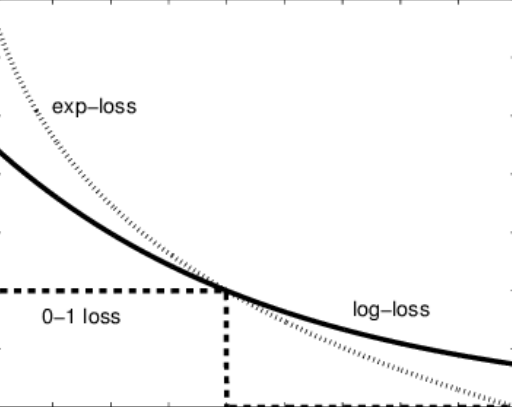
\includegraphics[width=6cm, height=5cm]{loss}
\end{center}
\hspace*{4ex}The squared error would not be a good choice for classification, primarily because it is not a monotonically decreasing function of $yf(x)$. However, there is a modification of this function, the \emph{Huber loss function}, which is more resistant to outliers and is used for both classification and regression.\\
Huber loss function for regression has the following form:
\[
    L_{\delta}(a)=
\begin{cases}
    \frac{1}{2}a^2,& \text{if } |a|\le\delta\\
    \delta(|a|-\frac{1}{2}\delta),& \text{otherwise }
\end{cases}
\]
while for the classification, it is:
\[
    L(y,f(x))=
\begin{cases}
   max(0,1-yf(x))^2,& \text{if } yf(x)\ge-1 \\
    -4yf(x),& \text{otherwise }
\end{cases}
\]
The figure below shows the relationship between the Huber, quadratic and absolute loss functions.
\begin{center}
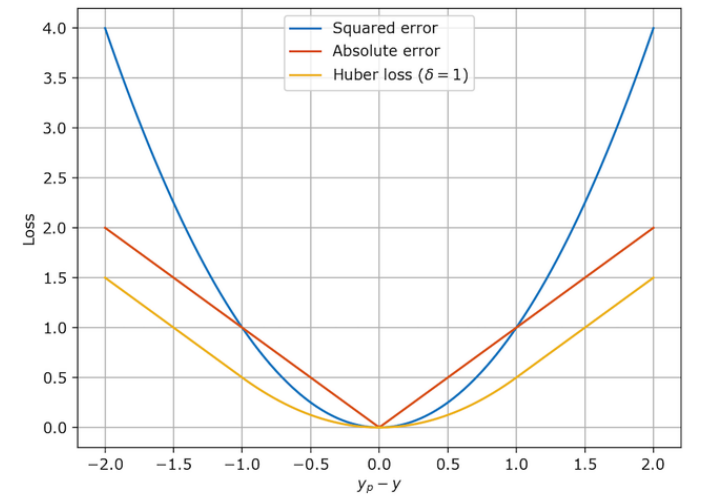
\includegraphics[width=8cm, height=6cm]{relation}
\end{center}

\begin{center}
\textbf{\large{\\4 “Off-the-Shelf” Procedures for Data Mining}\\}
\end{center}
\begin{center}
\textbf{\large{4.1 Introduction}\\}
\end{center}
\hspace*{4ex}Data mining is the process of discovering patterns in large data sets, using machine learning methods, statistics, and database systems.\\ 
\hspace*{4ex}Data mining applications can be demanding in terms of the problems they pose to learning procedures. The data is often very large, with many observations and variables. Also, the data are often unordered: they consist of a mixture of numerical and categorical variables, which usually have multiple factor levels. It happens that there are missing values or that the same data appears in more than one place. That is why, before finding a suitable model, the data is first arranged using methods of imputation, transformation, etc... Usually, only a certain portion of that data is actually meaningful for prediction, so it is very important not only to find a model that predicts well, but also to understand the data and what it shows. Therefore, models that are usually excellent for prediction, for example neural networks, are not the best choice for data mining. 
\hspace*{4ex}Due to the need for speed, easy interpretability and the generally messy nature of the data, there is a limitation in terms of using different models for prediction. An \emph{off-the-shelf} method is one that can be directly applied to the data without the need for preprocessing or adaptation.
\pagebreak
\begin{center}
\textbf{\large{\\4.2 Decision Trees}\\}
\end{center}
\hspace*{4ex}Decision trees best meet the requirements for data mining. They are relatively fast to model and provide a clear representation of the relationship between data (if they are not too large). Trees can be used on a mixture of numeric, categorical and binary data, and no imputation of missing data is required, thus freeing us from preprocessing. They are invariant to monotone data transformations, so there is no need for scaling. Another great advantage of trees is resistance to outliers.\\
\hspace*{4ex}The only drawback of trees that prevents them from being an ideal data mining tool is their imprecision. They rarely provide the precision that would be obtained using some other machine learning methods.\\
\hspace*{4ex}This problem is overcome by using boosting. Boosters drastically increase the accuracy of the model. Of course, increasing precision comes at a price: decreasing speed or interpretation. In the case of AdaBoost (Adaptive Boosting), speed, interpretation are lost, but resistance to overlapping data classes and mislabeling in the training set is also lost. The model with gradient boosting: \emph{gradient boosted mode} best maintains all the good sides of the trees, and better precision is obtained.
\begin{center}
\textbf{\large{\\5 Boosting Trees}\\}
\end{center}
\hspace*{4ex}Decision trees divide the predictor space into disjoint regions $R_j , j = 1, 2, ..., J$ which are represented by the end nodes of the tree. The constant $\gamma_j$ is assigned to each of the regions so that:
\begin{center}
$x\in R_j => f(x)=\gamma_j$
\end{center}
The tree can therefore be formally represented as:
\begin{equation*}
T(x;\Theta)=\sum_{j=1}^J\gamma_jI(x \in R_j),
\end{equation*}
with the parameter $\Theta=\{R_j,\gamma_j\}_1^J$ treated as hyperparameter. The parameters are found by minimizing the empirical risk
\begin{equation*}
\hat{\Theta}=argmin_{\Theta}\sum_{j=1}^J\sum_{x_i \in R_j}L(y_i,\gamma_i).
\end{equation*}
This is a significant combinatorial optimization problem and usually settles for approximate and sub-optimal solutions. It is useful to divide the problem into two parts:\\
\textbf{\\1. Finding $\gamma_j$ over the given $j$:} We usually use the mean value $y_i$ that falls into the region $R_j$, that is $\hat{\gamma_j}=\bar{y_i}$.\\
\textbf{\\2. Finding $R_j$:} Finding $R_j$ implies also finding $\gamma_j$. The method of top-down recursive partitioning is most often used. Additionally, it is sometimes necessary to find a smoother and more convenient approximation for $R_j$: 
\begin{equation*}
\tilde{\Theta}=argmin_{\Theta}\sum_{i=1}^N \tilde{L}(y_i,T(x_i,\Theta)).
\end{equation*}
Now we use $\hat{R_j}=\tilde{R_j}$ which gives us greater precision when finding $\gamma_j$.\\
\hspace*{4ex}The tree's \textbf{Gini index} is a measure of randomness in data sets. It aims to reduce the impurities (in terms of proper classification and partitioning) in the data, in the direction from the root nodes (at the top of the tree) to the leaf nodes (at the bottom of the tree) in the model. With the Gini index, it is possible to replace the loss obtained by wrong classification in tree growth. The boosting model is precisely the sum of such trees 
\begin{equation*}
f_M(x)=\sum_{m=1}^N T(x,\Theta_m).
\end{equation*}
induced in stages. In each step of this procedure it is necessary to calculate
\begin{equation*}
\hat{\Theta}_m=argmin_{\Theta}\sum_{i=1}^N L(y_i,f_{m-1}(x_i)+T(x_i;\Theta_m))
\end{equation*}
and the constants $\Theta_m=\{R_{jm},\gamma_{jm}\}_1^J$ of the next tree, assuming the current model $f_{m-1}(x)$.\\
\hspace*{4ex}When $R_{jm}$ is given, finding $\gamma_{jm}$ is straightforward:
\begin{equation*}
\hat{\gamma}_{jm}=argmin_{\gamma_{jm}}\sum_{x_i \in R_{jm}} L(y_i,f_{m-1}(x_i)+\gamma_{jm})
\end{equation*}
On the other hand, finding the $R_{jm}$ regions themselves is more difficult than with ordinary trees. The problem is simplified in some cases.\\
\hspace*{4ex}For the case when we have a quadratic loss function, the problem reduces to the tree that best predicts the residuals $y_i − f_{m−1}(x_i)$, where we get that $\hat{\gamma}_{jm}$ is the mean value of the residuals in the corresponding region.\\
\hspace*{4ex}In the case of exponential loss and two-class classification, the AdaBoost method is mostly used. With an absolute loss function, the solution is the median of the residuals of the corresponding region. For other criteria, there are fast iterative algorithms for finding $\hat{\gamma}_{jm}$, which give solid approximations. Simple and fast criteria for finding $\hat{\Theta}_m$ do not exist, so we decide on the approximation:
\begin{equation*}
\tilde{\Theta}=argmin_{\Theta}\sum_{i=1}^N \tilde{L}(y_i,T(x_i,\Theta)).
\end{equation*}

\begin{center}
\textbf{\large{6 Numerical Optimization via Gradient
Boosting}} 

\end{center}
\hspace*{4ex}Numerical optimization is a branch of mathematics and computer science that deals with finding the best solution for a specific problem in accordance with certain criteria. It may involve the minimization or maximization of a function or set of functions.\\
\hspace*{4ex}Fast algorithms approximating 
\begin{equation*}
\hat{\Theta}_{m}=argmin_{\Theta_{m}}\sum_{i=1}^N L(y_i,f_{m-1}(x_i)+T(x_i;\Theta_m))
\end{equation*}
for any differentiable loss function can be derived by their analogy with numerical optimization. The loss function when using $f(x)$ to predict $y$ on the training set is
\begin{equation*}
L(f)=\sum_{i=1}^N L(y_i,f(x_i)).
\end{equation*}
The goal is to reduce $L(f)$ with respect to $f$, where $f(x)$ is restricted to be the sum of trees $f_M(x)=\sum _{m=1}^M T(x;\Theta_m)$\\
\hspace*{4ex} Ignoring this limitation, the minimization of $L(f)$ can be understood as a numerical optimization
\begin{equation*}
\hat{f}=argmin_f L(f),
\end{equation*}
where the "parameters"\space $f \in R^N$ are the values of the approximating function $f(x_i)$ at each of the N points $f = \{f(x_1), f(x_2),...,f(x_N)\}^T$.\\
\hspace*{4ex} Numerical optimization methods solve
\begin{equation*}
\hat{f}=argmin_f L(f)
\end{equation*}
as a sum of component vectors $f_M=\sum_{m=0}^M h_m, h_m \in R^N$, where $f_0=h_0$ is the initial attempt, and each subsequent $f_m$ is induced based on $f_{m−1}$. Numerical optimization methods differ according to the method of calculating $h_m$ ("step").


\begin{center}
\textbf{\large{6.1  Steepest Descent}} 
\end{center}
\hspace*{4ex} Steepest Descent is an iterative optimization method. It is based on the idea that in each iteration we move in the direction of the greatest decrease of the function.\\
\hspace*{4ex} Specifically, for each iteration, the gradient of the function at the current point is determined and we move in the direction opposite to the gradient. This step is repeated until the algorithm converges to the minimum of the function.\\
\hspace*{4ex}The Steepest Descent method is often used to solve optimization problems in machine learning and other fields because it is simple to implement. However, there are also several drawbacks, such as slow convergence in cases with many dimensions.\\
The steepest descent method chooses $h_m=\rho_mg_m$, where $\rho_m$ is a scalar and $g_m \in R^N$ is gradient $L(f)$ calculated for $f=f_{m-1}$. The gradient components $g_m$ are
\begin{equation*}
g_{im}=[\frac{\partial L(y_i,f(x_i))}{\partial f(x_i)}]_{f(x_i)=f_{m-1}(x_i)}.
\end{equation*}
The step length $\rho_m$ is the solution for
\begin{equation*}
\rho_m=argmin_{\rho}L(f_{m-1}-\rho g_m)
\end{equation*}
The current solution is then updated to $f_m = f_{m−1}− \rho_m g_m$ and the process is repeated in the next iteration.
\pagebreak

\begin{center}
\textbf{\large{6.2 Gradient Boosting}}
\end{center}
\hspace*{4ex} \textbf{Gradient boosting} is one of the methods for numerical optimization. It uses the gradient of a function to determine the direction to move in each step.\\ 
\hspace*{4ex}Gradient boosting is an efficient method for finding optimal solutions for many optimization problems, but it has several drawbacks. For example, it may get stuck in local minimums or maximums, which means it will not find a globally optimal solution. Also, the learning rate plays an important role in the efficiency of gradient boosting and if it is too large, it can lead to divergence, and if it is too small, it can slow down the process of finding the optimal solution.\\
\hspace*{4ex}If minimizing the loss function
\begin{equation*}
L(f)=\sum_{i=1}^N L(y_i,f(x_i))
\end{equation*}
on the training set is the only goal, steepest descent would be the preferred strategy.\\
\hspace*{4ex}Gradient
\begin{equation*}
g_{im}=[\frac{\partial L(y_i,f(x_i))}{\partial f(x_i)}]_ {f(x_i)=f_{m-1}(x_i)}
\end{equation*}
from the previous chapter is defined only in the points $x_i$ of the training set, while the ultimate goal is the generalization of $f_M(x)$ to new data that are not represented in the training set. A possible solution is to induce the tree $T(x;\Theta_m)$ at the m-th place
iterations whose predictions $t_m$ are as close as possible to the negative gradient.\\
\hspace*{4ex} Using squared error we get:
\begin{equation*}
\Theta_m=argmin_{\Theta}\sum_{i=1}^N (-g_i m-T(x_i;\Theta))^2.
\end{equation*}
After constructing the previous tree, the corresponding constants in each region are given by:
\begin{equation*}
\hat{\gamma}_{jm}=argmin_{\gamma_{jm}}\sum_{x_i \in R_{jm}}L(y_i,f_{m-1}(x_i)+\gamma_{jm})
\end{equation*}
For classification: each tree $T_k^m$ is adapted to the corresponding negative gradient vector $g_{km}$,
\begin{equation*}
-g_{ikm}=[\frac{\partial L(y_i,f_1(x_1),...,f_K(x_i))}{\partial f_k(x_i)}]_{f(x_i)=f_{m-1}(x_i)}=I(y_i=G_k)-p_k(x_i)
\end{equation*}
so that
\begin{equation*}
p_k(x)=\frac{e^{f_k(x)}}{\sum_{l=1}^K e^{f_1 (x)}}
\end{equation*}
For binary classification (K = 2), only one tree is needed.

\begin{center}
\textbf{\large{6.3 Implementations of Gradient Boosting}}
\end{center}

\hspace*{4ex} We will now present the Gradient Boosting Algorithm.\\
Specific algorithms are obtained by inserting different loss criteria $L(y,f(x))$.
1. set $f_0(x)=argmin_{\gamma} \sum_{i=1}^N L(y_i,\gamma)$.\\\\
2. for values $m=1,...,M$:\\
\hspace*{4ex}(a)\space for values $i=1,...,N$ calculate:
\begin{equation*}
r_{im}=-[\frac{\partial L(y_i,f(x_i))}{\partial f(x_i)}]
\end{equation*}
\hspace*{4ex}(b)\space fit a regression tree to the targets $r_{im}$ giving terminal regions $R_{jm},j=1,2,...,J_m$.
\hspace*{4ex}(c)\space for values $j=1,...,J_m$ calculate:
\begin{equation*}
\gamma_{jm}=argmin_{\gamma}\sum_{x_i \in R_{jm}}L(y_i,f_{m-1}(x_i)+\gamma)
\end{equation*}\\
\hspace*{4ex}(d)\space update $f_m(x)=f_{m-1}(x)+\sum_{j=1}^{J_m} \gamma_{jm}I(x \in R_{jm})$.
3. output is $\hat{f}(x)=f_M(x)$\\
The first line of the algorithm is initialized to the optimal constant model, which is only one terminal node of the tree. The negative gradient components calculated in line 2(a) are called generalized or pseudo-residuals.\\
\hspace*{4ex}The classification algorithm is similar. Lines 2 (a)-(d) are repeated K times in each iteration m, once for each class using $−g_{i_{km}}$ from the previous section. The result in line 3 is K different (connected) extensions of the tree $f_{kM}(x),k=1,2,...,K$.\\
\hspace*{4ex}Gradient boosting as described here is implemented in the R gbm package (Ridgeway, 1999, \emph{"Gradient Boosted Models"}), and is freely available. Another R implementation of gradient boosting is mboost (Hothorn and B¨uhlmann, 2006)...
\begin{center}
\textbf{\large{7 Right-Sized Trees for Boosting}\\}
\end{center}
\hspace*{4ex}It is used to build decision trees with an optimal depth that is selected based on the data of the training set. This method differs from traditional boosting methods, such as AdaBoost, because it uses an algorithm to optimize the depth of the tree instead of increasing the weight of misclassified examples. This leads to better performance of the classifier compared to traditional methods. This method differs from traditional Boosting methods in that it uses "right-sized" trees instead of deep trees.\\
\hspace*{4ex}This method leads to less overfitting and better performance in cases with little data. This technique also allows for faster calculations and easier interpretation of results.\\
\hspace*{4ex} A simple approach is to constrain all trees to be \textbf{of the same size J}. Thus, J becomes a metaparameter of the entire boosting procedure that is adjusted to maximize the estimated performance for the current data set.\\
Possible values for J can be obtained by considering the properties of the objective function
\begin{equation*}
\eta=argmin_f E_{X,Y} L(Y,f(X)).
\end{equation*}
The objective function $\eta(x)$ is the one that has the lowest prediction risk on future data. That's the function we're trying to approximate. One important property of $\eta(x)$ is the degree of interaction of coordinate variables $X^T=(X_1,X_2,...,X_p)$ with each other. This is noted in its \textbf{ANOVA} (analysis of variance) expansion 
\begin{equation*}
\eta(X)=\sum_j \eta_j(X_j)+\sum_{jk} \eta_{jk}(X_j,X_k)+\sum_{jkl}\eta_{jkl}(X_j,X_k,X_l)+...
\end{equation*}
The first sum is over the functions of only one predictor variable $X_j$. The special functions $\eta_j(X_j)$ are those that together best approximate $\eta(X)$ under the loss criterion used. Each such $\eta_j(X_j)$ is called the \textbf{"main effect"} of $X_j$. The second sum represents second-order interactions, the third sum represents third-order interactions, and so on.\\
\hspace*{4ex} No interaction effects greater than $J-1$
are possible. A value of $J$ should be chosen that reflects the level of dominant interactions $\eta(x)$. Of course, it is mostly unknown, but in most situations it will tend towards low. Although in many cases $J=2$ will be insufficient, it is very unlikely that $J$ greater than 10 will be required. Experience so far indicates that $4 \le J \le 8$ works well in the context of boosting, and the results are quite insensitive to certain choices in this range. One can fine-tune the value of J by trying several different values and selecting the one that produces the lowest risk on the validation sample.
\begin{center}
\textbf{\large{8 Regularization}\\}
\end{center}
\hspace*{4ex} In addition to the size of the component trees, $J$, another meta-parameter of gradient boosting is the \textbf{number of boosting iterations $M$}. Each iteration typically reduces the training risk $L(f_M)$, so for M large enough this risk can be arbitrarily small. However, fitting the training data too well can lead to overfitting, which worsens the risk for future predictions. Therefore, there is an optimal number $M^*$ that minimizes the future risk. A practical way to estimate $M^*$ is to track the prediction risk as a function of $M$ on the validation sample. The value of $M$ that minimizes this risk is considered the estimate of $M^*$.\\
\begin{center}
\textbf{\large{8.1 Shrinkage}\\}
\end{center}
\hspace*{4ex} Controlling the value of $M $is not the only possible regularization strategy. The simplest implementation of downscaling in the context of boosting is to \emph{scale the contribution of each tree by a factor} $0 < \nu < 1$ when added to the current approximation.\\
\hspace*{4ex}Smaller values of $\nu$ (more downscaling) result in higher training risk for the same number of iterations $M$. Therefore, both $\nu$ and $M$ control the prediction risk on the training data. However, these parameters do not act independently. Smaller values of $\nu$ lead to larger values of $M$ for the same training risk, so there is a trade-off between the two.
\begin{center}
\textbf{\large{8.2 Subsampling}}
\end{center}
\hspace*{4ex}The idea is that at each iteration of the algorithm, a fraction $\eta$ of the training data (without repetition) is taken to be used to grow the next tree. This technique is called \emph{stochastic gradient boosting} (Friedman, 1999). A typical value for $\eta$ can be $\frac{1}{2}$, although for large $N$, $\eta$ can be significantly less than $\frac{1}{2}$.\\
\hspace*{4ex}Using \textbf{subsampling} reduces the computational time, but also in many cases provides a more accurate model. The downside is that we now have four parameters to set: $J$, $M$, $\nu$ and $\eta$. Usually, some earlier research determines appropriate values for $J$, $\nu$, and $\eta$, leaving $M$ as the main parameter.
\begin{center}
\textbf{\large{9 Interpretation}}
\end{center}
\hspace*{4ex}Single decision trees are very interpretive. The whole model can be completely represented by a simple two-dimensional graphic (binary tree) that is easy to visualize.
\begin{center}
\textbf{\large{9.1 Relative Importance of Predictor Variables}}
\end{center}
\hspace*{4ex} It is often useful to learn the relative importance or contribution of each input variable in predicting the response.\\
\hspace*{4ex}For a single decision tree T, Breiman (1984) suggested
\begin{equation*}
I_l^2(T)=\sum_{t=1}^{J-1} \hat{\iota}_t^2 I(v(t)=l)
\end{equation*}
as a measure of importance for each predictive variable $X_l$. The sum is over $J-1$ internal nodes of the tree. At each such node $t$, one of the input variables $X_{v(t)}$ is used to divide the region into two subregions; a special constant response is fitted within each. The particular variable chosen is the one that gives the maximum estimated improvement $\hat{i}_t^2$ in the squared error risk relative to a constant fit over the entire region. The squared relative importance of the variable $X_l$ is the sum of such squared improvements at all internal nodes for which it is chosen as the partition variable.\\
\hspace*{4ex} For K-class classification, $K$ separate models $f_k(x),k=1,2,...,$K are induced, each of which consists of a sum of trees $f_k(x)=\sum_{m=1}^M T_{km}(x)$.\\
\begin{center}
\textbf{\large{9.2 Partial Dependence Plot (PDP)}}
\end{center}
\hspace*{4ex}Plotting $f(X)$ as a function of its arguments provides an overview of the dependence of $f(X)$ on the common value of the input variables. Unfortunately, such visualization is limited to lower dimensional views. We can easily show functions of one or two arguments, either continuous, discrete or combined. For more than two or three variables a useful alternative can sometimes be to display a collection of plots, each showing the partial dependence of the approximation $f(X)$ on a selected small subset of the input variables. Example:
\begin{equation*}
\eta(X)=\sum_j \eta_j(X_j)+\sum_{jk} \eta_{jk}(X_j,X_k)+\sum_{jkl}\eta_{jkl}(X_j,X_k,X_l)+...
\end{equation*}
\hspace*{4ex} Consider a subvector $X_S$ of $l<p$ input variables $X_T=(X_1, X_2,...,X_p)$, indexed by $S\subset 1,2,...,p$. Let $S \cup C = 1, 2, ..., p$. The general function $f(X)$ will depend on all input variables: $f(X)=f(X_S,X_C)$. The partial dependence of $f(X)$ on $X_S$ is: $f_S(X_S) = E_{X_C} f(X_S,X_C)$.\\
\hspace*{4ex}The partial dependence function is estimated by calculating the average on the training data (\emph{Monte Carlo method}):
\begin{equation*}
\hat{f_S}(X_S)=\frac{1}{N}\sum_{i=1}^N f(X_S,x_{iC}),
\end{equation*}
where $x_{1C}, x_{2C},...,x_{NC}$ are the values of $X_C$ occurring in the training set.\\
\hspace*{4ex} \textbf{PDP} are a simple and intuitive way to visualize relationships between variables and can be a valuable tool for gaining a deeper understanding of complex machine learning models. It is a \emph{global method}: The method considers all instances and talks about the global relationship of some characteristic with the predicted outcome. It is useful for questions such as: How much of the wage gap between men and women is due solely to gender, as opposed to differences in education or work experience?

\begin{center}
\textbf{\large{10 Literature}}
\end{center}
1. Trevor Hastie, Robert Tibshirani, Jerome Friedman (2017), The Elements of Statistical Learning, second edition; corrected 12th printing.\\
2. Mladen Nikolić, Anđelka Zečević (2019,) Mašinsko učenje\\
3. Simon Kornblith, Honglak Lee, Ting Chen, Mohammad Norouzi (2020), Demystifying Loss Functions for Classification\\
https://openreview.net/forum?id=jNTeYscgSw8\\
4. Vishal Rajput, Robustness of different loss functions and their impact on network’s learning capability, Computer Science Department, KU Leuven, Belgium\\
https://arxiv.org/abs/2110.08322\\
5. D. Baehrens, T. Schroeter, S. Harmeling, M. Kawanabe, K. Hansen, K.-R. Müller (2010), How to Explain Individual Classification Decisions, Journal of Machine Learning Research 11 1803-1831\\
https://www.jmlr.org/papers/volume11/baehrens10a/baehrens10a.pdf\\
6. David Rosenberg, Machine learning course materials\\
http://github.com/davidrosenberg/mlcourse\\
7. A. Lahiri, B. Paria, P. K. Biswas, Forward Stagewise Additive Model for Collaborative Multiview Boosting\\
https://arxiv.org/pdf/1608.01874.pdf\\
8. Yoav Freund, Robert E. Schapire, ATT Labs Research, A Short Introduction to Boosting\\
https://cseweb.ucsd.edu/~yfreund/papers/IntroToBoosting.pdf\\
9. Christoph M., Partial Dependence Plot (PDP)\\
https://christophm.github.io/interpretable-ml-book/pdp.html\\
10. Dan S. Becker, Partial Dependence Plots\\
https://www.kaggle.com/code/dansbecker/
partial-dependence-plots/notebook\\
11. Akancha Tripathi, A Detailed Guide On Gradient Boosting Algorithm With Examples\\
https://www.analytixlabs.co.in/blog/gradient-boosting-algorithm/
\end{document}





